\documentclass[tikz,border=2pt]{standalone}
\usepackage{amsmath}
\usepackage{pgfplots}
\pgfplotsset{compat=1.18}
\usetikzlibrary{arrows.meta}
\begin{document}
% Four dplyr verbs on the 2021 rows (Country, Year, Transport) of the emissions extract:
% select keeps columns, filter keeps rows, mutate appends Big = Transport > 100 (FALSE, TRUE, FALSE), arrange(desc()) reorders 24, 148, 31 -> 148, 31, 24.
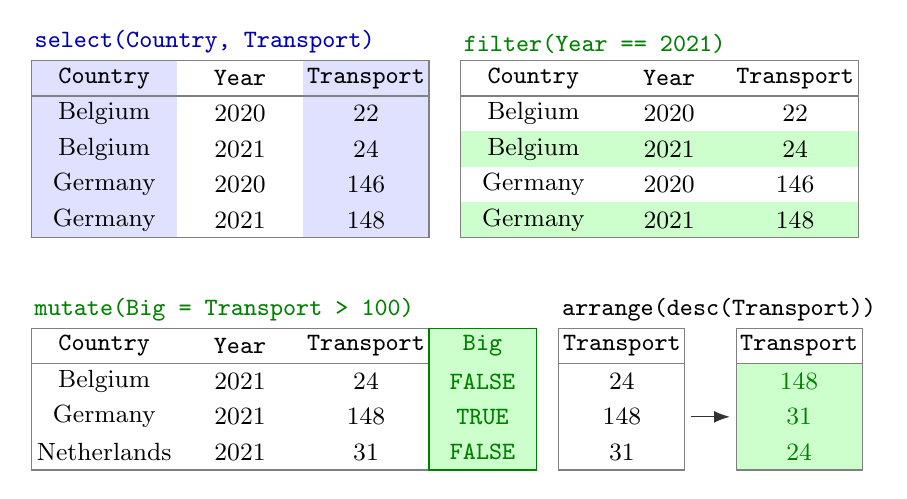
\begin{tikzpicture}[font=\small, >={Latex[length=2mm]},
  title/.style={anchor=south west, font=\small\ttfamily, inner sep=1pt},
  hd/.style={font=\small\ttfamily}]
  \def\w{1.6}  % width of Year and Transport columns
  \def\wa{1.85} % width of the Country column
  \def\h{0.45} % row height
  % a 3-column table with header, rows given as {country/year/transport}
  \newcommand{\tbl}[3]{% #1 origin, #2 rows, #3 number of rows
    \begin{scope}[shift={#1}]
      \node[hd] at (0.5*\wa,0) {Country};
      \node[hd] at (\wa+0.5*\w,0) {Year};
      \node[hd] at (\wa+1.5*\w,0) {Transport};
      \foreach \c/\y/\t [count=\i] in {#2} {
        \node at (0.5*\wa,-\i*\h) {\c};
        \node at (\wa+0.5*\w,-\i*\h) {\y};
        \node at (\wa+1.5*\w,-\i*\h) {\t};
      }
      \draw[gray] (0,-0.5*\h) -- (\wa+2*\w,-0.5*\h);
      \draw[gray] (0,0.5*\h) rectangle (\wa+2*\w,-#3*\h-0.5*\h);
    \end{scope}}
  % ---- select ----
  \begin{scope}[shift={(0,0)}]
    \fill[blue!12] (0,0.5*\h) rectangle (\wa,-4.5*\h);
    \fill[blue!12] (\wa+\w,0.5*\h) rectangle (\wa+2*\w,-4.5*\h);
    \tbl{(0,0)}{Belgium/2020/22,Belgium/2021/24,Germany/2020/146,Germany/2021/148}{4}
    \node[title, blue!70!black] at (0,0.5*\h+0.05) {select(Country, Transport)};
  \end{scope}
  % ---- filter ----
  \begin{scope}[shift={(5.45,0)}]
    \fill[green!20] (0,-1.5*\h) rectangle (\wa+2*\w,-2.5*\h);
    \fill[green!20] (0,-3.5*\h) rectangle (\wa+2*\w,-4.5*\h);
    \tbl{(0,0)}{Belgium/2020/22,Belgium/2021/24,Germany/2020/146,Germany/2021/148}{4}
    \node[title, green!50!black] at (0,0.5*\h+0.05) {filter(Year == 2021)};
  \end{scope}
  % ---- mutate ----
  \begin{scope}[shift={(0,-3.4)}]
    \fill[green!20] (\wa+2*\w,0.5*\h) rectangle (\wa+2.85*\w,-3.5*\h);
    \tbl{(0,0)}{Belgium/2021/24,Germany/2021/148,Netherlands/2021/31}{3}
    \draw[green!50!black] (\wa+2*\w,0.5*\h) rectangle (\wa+2.85*\w,-3.5*\h);
    \node[hd, green!50!black] at (\wa+2.425*\w,0) {Big};
    \foreach \v [count=\i] in {FALSE,TRUE,FALSE} \node[green!50!black] at (\wa+2.425*\w,-\i*\h) {\texttt{\v}};
    \node[title, green!50!black] at (0,0.5*\h+0.05) {mutate(Big = Transport > 100)};
  \end{scope}
  % ---- arrange ----
  \begin{scope}[shift={(6.7,-3.4)}]
    \node[hd] at (0.5*\w,0) {Transport};
    \foreach \t [count=\i] in {24,148,31} \node at (0.5*\w,-\i*\h) {\t};
    \draw[gray] (0,-0.5*\h) -- (\w,-0.5*\h);
    \draw[gray] (0,0.5*\h) rectangle (\w,-3.5*\h);
    \begin{scope}[shift={(\w+0.65,0)}]
      \fill[green!20] (0,-0.5*\h) rectangle (\w,-3.5*\h);
      \node[hd] at (0.5*\w,0) {Transport};
      \foreach \t [count=\i] in {148,31,24} \node[green!50!black] at (0.5*\w,-\i*\h) {\t};
      \draw[gray] (0,-0.5*\h) -- (\w,-0.5*\h);
      \draw[gray] (0,0.5*\h) rectangle (\w,-3.5*\h);
    \end{scope}
    \draw[->, gray!40!black] (\w+0.08,-2*\h) -- (\w+0.57,-2*\h);
    \node[title] at (0,0.5*\h+0.05) {arrange(desc(Transport))};
  \end{scope}
\end{tikzpicture}
\end{document}
